\begin{center}
\textbsc{Réponses}
\end{center}

\everymath{\textstyle}
\begin{enumerate}[label=\thechapter.\arabic*, font=\bfseries, itemsep=7mm,labelsep*=3mm,left=0mm]
%1
\item 
$\nombre{91239123}=\nombre{8924}\cdot \nombre{10224}+147$
%$\numprint{91239123}$



%2
\item
Le quotient est $-6$ et reste est $1$.

\item 


\begin{enumerate}[label=\alph*),itemsep=0mm,left=0mm]
	\item  \textbf{Divisions euclidiennes}
	\begin{enumerate}
		\item[\textbf{1)}] Pour $23$ par $4$ : \\
		On cherche $q$ et $r$ tels que $23 = 4 \cdot q + r$ avec $0 \le r < 4$. \\
		$$23 = 4 \cdot 5 + 3$$
		Le quotient est $q = 5$ et le reste est $r = 3$.
		
		\item[\textbf{2)}] Pour $-23$ par $4$ : \\
		Le reste doit vérifier $0 \le r < 4$. \\
		On a $-23 = 4 \cdot (-5) - 3 = 4 \cdot (-5) - 4 + 1 = 4 \cdot (-6) + 1$.
		$$-23 = 4 \cdot (-6) + 1$$
		Le quotient est $q = -6$ et le reste est $r = 1$.
	\end{enumerate}
	
	\item  \textbf{Recherche des deux entiers naturels}
	
	Soient $a$ et $b$ deux entiers naturels. Supposons $a > b$.
	\begin{itemize}
		\item La différence est $538 \implies a - b = 538 \implies a = b + 538$.
		\item La division euclidienne de $a$ par $b$ donne : $a = 13 \cdot b + 34$ (avec $34 < b$).
	\end{itemize}
	
	On égalise les deux expressions de $a$ :
	$$13b + 34 = b + 538$$
	$$12b = 504$$
	$$b = \frac{504}{12} = 42$$
	
	On vérifie que la condition sur le reste est respectée ($34 < 42$). \\
	On calcule ensuite $a$ :
	$$a = 42 + 538 = 580$$
	
	Les deux entiers naturels sont \textbf{$580$} et \textbf{$42$}.
	
	\item  \textbf{Détermination de l'entier naturel $n$}
	
	Soit $q$ le quotient commun. Traduisons les deux divisions euclidiennes de $n$ :
	\begin{itemize}
		\item Par $23$ : $n = 23 \cdot q + 1$
		\item Par $17$ : $n = 17 \cdot q + 13$
	\end{itemize}
	
	On égalise les deux expressions de $n$ :
	$$23q + 1 = 17q + 13$$
	$$6q = 12$$
	$$q = 2$$
	
	On en déduit la valeur de $n$ :
	$$n = 23 \cdot 2 + 1 = 47$$
	(\textit{Vérification avec la 2\textsuperscript{e} division :} $17 \cdot 2 + 13 = 34 + 13 = 47$).
	
	L'entier naturel $n$ recherché est \textbf{$47$}.
	
	\item \textbf{Recherche des restes et des valeurs de $x$}
	
	La division euclidienne de $x$ par $3$ a pour quotient $7$ :
	$$x = 3 \cdot 7 + r = 21 + r \quad \text{avec} \quad 0 \le r < 3$$
	
	\begin{itemize}
		\item Le diviseur étant $3$, les restes possibles sont : \textbf{$r \in \{0, 1, 2\}$}.
		\item On en déduit les valeurs possibles pour $x$ :
		\begin{itemize}
			\item Si $r = 0$, $x = 21 + 0 = 21$
			\item Si $r = 1$, $x = 21 + 1 = 22$
			\item Si $r = 2$, $x = 21 + 2 = 23$
		\end{itemize}
	\end{itemize}
	
	Les valeurs de $x$ possibles sont \textbf{$21$, $22$ et $23$}.
\end{enumerate}


%3
\item 
\begin{tasks}[after-item-skip=2mm,item-indent=5mm,column-sep=2mm](4)
\task $12$
\task $32$
\task $52$
\end{tasks}



%4
\item 
Les restes possibles sont $0\pvirg{0.5} 1\pvirg{0.5} 2$. Les valeurs possibles pour $n$ sont $21\pvirg{0.5} 22\pvirg{0.5} 23$.



%5
\item 
$a=18q+13=6\cdot(3q)+6\cdot 2 +1=6\cdot(3q+2)+1$.\eh{2} Le reste est donc de $1$.


\setlength{\itemsep}{10mm}
%6
\item 
\begin{enumerate}[label=\alph*)]\setlength{\itemsep}{4mm}
\item Le nombre $n(n+1)(n+2)(n+3)$ est le produit de 4 nombres consécutifs. Parmi eux, il y a donc forcément un multiple de $2$, un multiple de $3$ est encore un multiple $4$. Le nombre initial est donc forcément un multiple de $2\cdot 3 \cdot 4 =24$.
\item Même raisonnement.
\end{enumerate}



%7
\item 
On veut $a=5(3r)+r=16r$ \, avec $r\in\{0;1;2;3;4\}$.

\smallskip
Donc : \eh{2} $a=0 \ou{5} a=16 \ou{5} a=32 \ou{5} a=48 \ou{5} a=64$




%8
\item Il faut se rappeler que le reste d'une division doit être plus petit que le diviseur. Nous obtenons alors :
\begin{enumerate}[label=\alph*)]\setlength{\itemsep}{4mm}
\item $\bm{842}=256\cdot 3 +\fbox{$74$}$ (division de $842$ par $256$).

\smallskip
Puis on écrit $\nombre{96842}=256 \cdot 375+\bm{256\cdot 3+74}=256\cdot 378+\fbox{74} $
\item $\bm{842}=375\cdot 2 +\fbox{$92$}$ (division de $842$ par $375$).

\smallskip
Puis on écrit $\nombre{96842}=256 \cdot 375+\bm{375\cdot 2 +92}=258\cdot 375+\fbox{$92$} $
\end{enumerate}




%9
\item Dans ce qui suit, $k$ et $m$ sont des nombres entiers $(\in \Z)$.

\begin{enumerate}[label=\alph*)]\setlength{\itemsep}{4mm}
\item Soit $n=2k+1$ un nombre entier impair. Alors $n^2=4k^2+4k+1=4 k (k+1)+1$.

\smallskip
Nous avons que soit $k$ soit $k+1$ est pair et par conséquent $k(k+1)=2m$.

\smallskip
Donc $n^2=4\cdot 2m +1 = 8m+1$ et le reste de la division de $n^2$ par 8 est de 1.
\item Soit $n=2k$ un nombre entier pair. Alors $n^2=4k^2$ et deux cas sont possibles :

\smallskip
\textbf{$\bm{k}$ est pair :} $k=2m$ donc $n^2=4\cdot(2m)^2=16m^2=8\cdot(2m^2)+\fbox{$0$}$\\
\phantom{\textbf{$\bm{k}$ est pair :}} On conclut que $n^2$ est un multiple de 8.

\vspace{-2mm}
\textbf{$\bm{k}$ est impair :} $k=2m+1$ donc $n^2=4(4m^2+4m+1)=16m^2+16m+4=8\overbrace{(2m^2+2m)}^{quotient}+\fbox{$4$}$\\
\phantom{\textbf{$\bm{k}$ est impair :}} Donc le reste de la division de $n^2$ par 8 est 4 car $0\leqslant 4 < 8$.
\end{enumerate}
\pagebreak



%10
\item
En pratique, il serait possible de résoudre cet exercice en résolvant l'équation de manière conventionnelle, à savoir en égalant à 0 et en factorisant.

\smallskip
Voici une autre manière de voir ce problème en \guillemets{dénombrant} les possibilités. Ce procédé se révélera utile dans d'autres cas de figure.

\begin{enumerate}[label=\alph*)]\setlength{\itemsep}{4mm}
\item $n^2+n=20 \ssi[2] n(n+1)=20$. 

\smallskip
Voici les couples de nombres entiers dont le produit est 20 : 
$$(\pm 1;\pm 20) \eh{5} (\pm 2;\pm 10) \eh{5} (\pm 4;\pm 5)$$
Les seuls qui soient consécutifs sont $(4; 5)$ et $(-5; -4)$. \,Les solutions sont donc $n=4$ et $n=-5$.

\item $n^2+2n=35 \ssi[2] n(n+2)=35$. 

\smallskip
Voici les couples de nombres entiers dont le produit est 35 : 
$$(\pm 1;\pm 35) \eh{5} (\pm 5;\pm 7)$$
Les couples qui vérifient la condition sont $(5; 7)$ et $(-7; -5)$. \,Les solutions sont donc $n=5$ et $n=-7$.
\end{enumerate}



%11
\item
Nous avons $x^2-2xy=15 \ssi[2] x(x-2y)=15$.

\smallskip
Voici les couples de nombres entiers positifs dont le produit est 15 : 
$$(1; 15) \eh{5} (3 ; 5)$$
En remarquant que $x$ est forcément plus grand que $(x-2y)$, nous pouvons construire le tableau suivant qui résume toutes les possibilités :

\begin{center}
\begin{tabular}{|c||c||c|}
\hline
$x$		& $15$	& $5$\\ 
\hline
$x-2y$	& $1$	& $3$\\
\hline
\rowcolor{gray!40} $x(x-2y)$	& $15$	& $15$\\
\hline\hline
$x$		& $15$	& $5$\\
\hline
$y$		& $7$	& $1$\\
\hline
\end{tabular}
\end{center}
Les solutions sont donc $(15; 7)$ et $(5; 1)$. \,D'où : $S=\big\lbrace(5; 1) \; ; \; (15; 7)\big\rbrace$
	



%%11
%\item
%A l'aide de la décomposition en nombre premiers, déterminer le pgcd des nombres suivants :
%\begin{enumerate}[label=\alph*)]\setlength{\itemsep}{3mm}
%\item $126=2\cdot 3^2\cdot 7$\\
%$230=2\cdot 5\cdot 23$
%
%\smallskip
%Donc $\pgcd(126\; ;230)=2$
%\item $390= 2\cdot 3\cdot 5 \cdot 13$ \\
%$720=2^4\cdot 3^2\cdot 5$ \\
%$450=2\cdot 3^2 \cdot 5^2$
%
%\smallskip
%Donc $\pgcd(390\; ;720\; ;450)=2\cdot 3\cdot 5=30$
%\item $\pgcd(180\; ; 606\; ; 750)=6$.
%\end{enumerate}



%12
\item
\begin{enumerate}[label=\roman*),itemsep=5mm]
\item $(n+1)^3=n^3+3n^2+3n+1=n^2(n+3)+3n+1$.
\item Le reste de division de $(n+1)^3$ par $n^2$ vaut $(3n+1)$ si et seulement si $$0\leqslant 3n+1<n^2$$


D'une part : $0\leqslant 3n+1 \ssi[2] -1\leqslant 3n \ssi -\frac{1}{3}\leqslant n$

\medskip
D'autre part : $3n+1<n^2 \ssi[2] n^2-3n-1>0 \ssi[2] \left(n-\frac{3-\sqrt{13}}{2}\right)\left(n-\frac{3+\sqrt{13}}{2}\right)>0 $

\begin{center}\begin{tikzpicture}[baseline=(current bounding box.north)]
\tikzset{t style/.style = {style = densely dashed}}
   \tkzTabInit[lgt=3,espcl=3]{$\boldsymbol{n}$/0.7 , $\left(n-\frac{3-\sqrt{13}}{2}\right)$/0.9 , $\left(n-\frac{3+\sqrt{13}}{2}\right)$/0.9 , $\boldsymbol{E(n)}$/0.7}{$\scriptstyle -\infty$ , $\textstyle\frac{3-\sqrt{13}}{2}$ , $\textstyle\frac{3+\sqrt{13}}{2}$, $\scriptstyle +\infty$}
%   \tkzTabLine{  ,  -  , t , - , }
   \tkzTabLine{  ,  -  , z , + , t , +}
   \tkzTabLine{  ,  -  , t , - , z , + }
   \tkzTabLine{  ,  +  , 0 , - , 0 , + }
%   \tkzTabLine{  ,  \decroi , A.V. , \decroi , }
   \draw[->=stealth, line width=1.5pt] (T11) -> (T21.east) node[right=2pt] {$\R$};
   \draw[double, line width=1.5pt] (T03) -> (T23) ;
%   \draw[line width=1.5pt] (T05) -> (T25) ;
\end{tikzpicture}\end{center}


\medskip
\everymath{\textstyle}
Comme $\frac{3-\sqrt{13}}{2}\simeq -0.3$ \et{1} $\frac{3-\sqrt{13}}{2}\simeq 3.3$, sachant que $n$ est un entier, les 2 conditions ci-dessus seront remplie pour $n\geqslant 4$.

\smallskip
Le reste de division de $(n+1)^3$ par $n^2$ vaut $(3n+1)$ si et seulement si $n\geqslant 4$.
\end{enumerate}



%13
\item
Il faut compléter l'algorithme d'Euclide. On part du dernier reste non-nul (qui est le pgcd) et on suit le sens des flèches en remontant l'algorithme pour compléter les opérations :


\hspace{6cm}\begin{minipage}[t][][b]{0.5\textwidth}
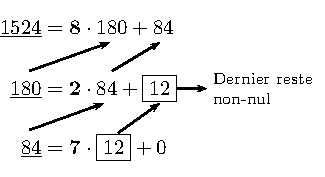
\includegraphics[scale=1]{Chapitre_2_arithmetique/figures/Correction/fig_co_1/fig_co_1.pdf}
\end{minipage}


On obtient $a=1524$ et $b=180$.




%14
\item
\begin{enumerate}[label=\alph*),itemsep=4mm]
\item 
Calculons $\pgdc(9945;3003)$ :

\hspace{6cm}\begin{minipage}[t][][b]{0.5\textwidth}
\vspace{-11.5mm}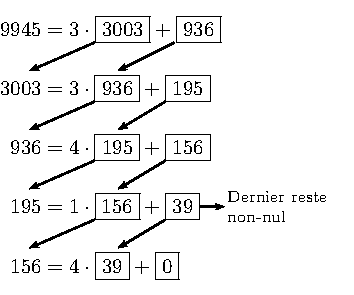
\includegraphics[scale=1]{Chapitre_2_arithmetique/figures/Correction/fig_co_2/fig_co_2.pdf}
\end{minipage}

\smallskip
Donc $\pgdc(9945;3003)=39$
\item 
$\pgdc(18480;9828)=84$
\item Par propriété du $\text{pgcd}$, pour tout entier $a$, $\text{pgcd}(-a; b) = \text{pgcd}(a; b)$.  

On a donc $\text{pgcd}(-286; 390) = \text{pgcd}(286; 390)$.

On effectue les divisions euclidiennes successives :
\begin{align*}
	390 &= 286 \cdot 1 + 104 \\
	286 &= 104 \cdot 2 + 78 \\
	104 &= 78 \cdot 1 + 26 \\
	78 &= 26 \cdot 3 + 0
\end{align*}

Le dernier reste non nul est $26$.  
Ainsi, $\text{pgcd}(-286; 390) = 26$.
\end{enumerate}


%EXERCICE
\item
\begin{itemize}\item[1)] Non car $\operatorname{PGCD}(4847 ; 5633)=131$
	
	$$
	\begin{aligned}
		5633 & =4847 \cdot 1+786 \\
		4847 & =786 \cdot 6+131 \\
		786 & =131 \cdot 6
	\end{aligned}
	$$
	
	\item[2)] Oui car $\operatorname{PGCD}(5617 ; 813)=1$
	
	$$
	\begin{aligned}
		5617 & =813 \cdot 6+739 \\
		813 & =739 \cdot 1+74 \\
		739 & =74 \cdot 9+73 \\
		74 & =73 \cdot 1+1
	\end{aligned}
	$$
\end{itemize}


%EXERCICE
\item $324=12 \cdot 27=12 \cdot 3^3$
$n$ doit être un multiple de 12 , mais pas un multiple de 36 sinon le $\operatorname{PGCD}(n ; 324)$ serait supérieur ou égal à 36 . Les entiers $n$ appartiennent à l'ensemble :
$\{12 ; 24 ; 48 ; 60 ; 84 ; 96 ; 120 ; 132 ; 156 ; 168 ; 192\}$.


%EXERCICE
\item On cherche le diviseur $b>9$ tel que :

$$
\left\{\begin{array} { l } 
	{ 1 8 0 9 = b q + 9 } \\
	{ 2 5 2 7 = b q ^ { \prime } + 7 }
\end{array} \Leftrightarrow \left\{\begin{array}{l}
	1800=b q \\
	2520=b q^{\prime}
\end{array} \Leftrightarrow\right.\right.
$$

$b>9$ et divise $\operatorname{PGCD}(4284 ; 3510)=360$
Le plus grand diviseur $b$ possible est donc 360 .



%15
\item\label{exer:pgdc_et_produit}
On note $(a;b)$ les couples de nombre entier de pgcd 14 et tels que $ab=7056$. Alors :
\begin{center}
$\left.\begin{tabular}{r}
$a=14\cdot a'$\\
$b=14\cdot b'$
\end{tabular}\right\rbrace$ avec $a'$ et $b'$ premiers entre eux.\end{center}
Comme $a\cdot b=7056$ alors $a'\cdot b'=\frac{7056}{14\cdot 14}=36$.

\medskip
Les possibilités pour $a'$ et $b'$ sont donc:
$$\boxed{\pt{1}{36}} \pvirg{4} \xcancel{\pt{2}{18}} \pvirg{4} \xcancel{\pt{3}{12}} \pvirg{4} \boxed{\pt{4}{9}} \pvirg{4} \xcancel{\pt{6}{6}}$$

Les couples qui ne sont pas premiers entre-eux ont étés barrés. Il reste donc 2 possibilités :
\renewcommand{\arraystretch}{1.4}
$$\begin{array}{r c l}
\pt{1}{36}& \overset{\cdot 14}{\longrightarrow} & \pt{14}{504} \\
\pt{4}{9} & \overset{\cdot 14}{\longrightarrow}  & \pt{56}{126}
\end{array}$$
Il y a alors deux couples vérifiant les conditions : $\pt{14}{504}$ et $\pt{56}{126}$.



%16
\item 
\begin{multicols}{2}
	\begin{enumerate}[label=\roman*),itemsep=5mm,left=-1mm,labelsep*=2mm]
		\item $3412=4\cdot 853+0$\\
		Donc $3412\equiv 0 \pmod{4}$
		\item $177=9\cdot 19+6$\\
		Donc $177\equiv 6 \pmod{9}$
		\item $31=31\cdot 1+0$\\
		Donc $31\equiv 0 \pmod{31}$
		\item $31=25\cdot 1+6$\\
		Donc $31\equiv 6 \pmod{25}$
		\item $365=5\cdot 73+0$\\
		Donc $365\equiv 0 \pmod{5}$
		\item $-3122=3\cdot (-1041)+1$\\
		Donc $-3122\equiv 1 \pmod{3}$
		\item $\nombre{31458687312}=10\cdot 3145868731+2$\\
		Donc $\nombre{31458687312}\equiv 2 \pmod{10}$
		\item $\nombre{-259874629}=10\cdot (-25987463)+1$\\
		Donc $\nombre{-259874629}\equiv 1 \pmod{10}$
	\end{enumerate}
\end{multicols}

%17
\item 
\begin{enumerate}[label=\roman*),itemsep=5mm,left=-1mm,labelsep*=2mm]
	\item[\textbf{a)}] \textbf{Vrai.} \\
	\textit{Justification :} $471 - 11 = 460$. Or $460 = 23 \cdot 20$, ce qui signifie que $23 \mid (471 - 11)$.
	
	\item[\textbf{b)}] \textbf{Faux.} \\
	\textit{Justification :} $370 - 17 = 353$. Or $353 = 13 \cdot 27 + 2$, donc $13 \nmid (370 - 17)$. \\
	(\textit{Autre méthode :} $370 = 13 \cdot 28 + 6 \implies 370 \equiv 6 \pmod {13}$ et $17 = 13 \cdot 1 + 4 \implies 17 \equiv 4 \pmod {13}$. Comme $6 \neq 4$, l'affirmation est fausse).
	
	\item[\textbf{c)}] \textbf{Vrai.} \\
	\textit{Justification :} $29 - (-121) = 29 + 121 = 150$. Or $150 = 5 \cdot 30$, donc $5 \mid (29 - (-121))$.
	
	\item[\textbf{d)}] \textbf{Faux.} \\
	\textit{Justification :} $-30 - (-1) = -30 + 1 = -29$. Or $-29$ n'est pas un multiple de $26$.
	
	\item[\textbf{e)}] \textbf{Vrai.} \\
	\textit{Justification :} Par définition de la congruence :
	\begin{itemize}
		\item $914 - 21 = 19 \cdot 47$, donc $19 \mid (914 - 21)$, d'où $914 \equiv 21 \pmod {19}$.
		\item De même, $47 \mid (914 - 21)$, d'où $914 \equiv 21 \pmod {47}$.
	\end{itemize}
	\textit{Remarque :} Bien que $21 \ge 19$ (ce n'est donc pas le reste de la division euclidienne par 19), l'égalité de congruence reste tout à fait exacte.
	
	\item[\textbf{f)}] \textbf{Vrai.} \\
	\textit{Justification :} Par définition, $b \equiv 0 \pmod a \iff b - 0 = k \cdot a \iff b = k \cdot a \iff a \mid b$.
	
	\item[\textbf{g)}] \textbf{Vrai.} \\
	\textit{Justification :} Si $b \equiv 0 \pmod a$ et $c \equiv 0 \pmod a$, alors $a \mid b$ et $a \mid c$. Par propriété de la divisibilité, $a$ divise toute combinaison linéaire $\alpha b + \beta c$ pour tous entiers $\alpha, \beta$, d'où $\alpha b + \beta c \equiv 0 \pmod a$.
\end{enumerate}

\item

\begin{itemize}
	\item \textbf{Étude de $351$ :}
	$$351 = 7 \cdot 50 + 1 \implies 351 \equiv 1 \pmod 7$$
	Par compatibilité avec les puissances :
	$$351^{12} \equiv 1^{12} \equiv 1 \pmod 7$$
	
	\item \textbf{Étude de $85$ :}
	$$85 = 7 \cdot 12 + 1 \implies 85 \equiv 1 \pmod 7$$
	Par compatibilité avec les puissances :
	$$85^{15} \equiv 1^{15} \equiv 1 \pmod 7$$
	
	\item \textbf{Produit :}
	Par compatibilité avec la multiplication :
	$$351^{12} \cdot 85^{15} \equiv 1 \cdot 1 \equiv 1 \pmod 7$$
\end{itemize}



% exo
\item

\begin{enumerate}
	\item \textbf{Étude du premier terme $5^{2n}$ :}
	On réécrit la puissance à l'aide des règles de calcul :
	$$5^{2n} = \left(5^2\right)^n = 25^n$$
	
	Or, $25 = 11 \cdot 2 + 3$, donc :
	$$25 \equiv 3 \pmod{11}$$
	
	Par compatibilité de la congruence avec les puissances, on a :
	$$5^{2n} \equiv 3^n \pmod{11}$$
	
	\item \textbf{Étude du second terme $14^n$ :}
	On effectue la division euclidienne de $14$ par $11$ :
	$$14 = 11 \cdot 1 + 3 \implies 14 \equiv 3 \pmod{11}$$
	
	Par compatibilité de la congruence avec les puissances, on a :
	$$14^n \equiv 3^n \pmod{11}$$
	
	\item \textbf{Soustraction des congruences :}
	Par compatibilité avec la soustraction :
	$$5^{2n} - 14^n \equiv 3^n - 3^n \pmod{11}$$
	$$5^{2n} - 14^n \equiv 0 \pmod{11}$$
\end{enumerate}

\textbf{Conclusion :} 
Pour tout entier naturel $n$, $5^{2n} - 14^n$ est divisible par $11$.


%17
\item
\begin{enumerate}[label=\roman*),itemsep=5mm,left=-1mm,labelsep*=2mm]
	\item $\phantom{195}1=13\cdot 0+1$\\
	$1951=13\cdot 150+1$\\
	$1964=13\cdot 151+1$\\
	$1977=13\cdot 152+1$\\
	$1990=13\cdot 153+1$ \eh{4} Donc, $1\equiv 1951 \equiv 1964 \equiv 1977 \equiv 1990 \pmod{13}$
	
	\item $1776=40\cdot 44+16$\\
	$1976=40\cdot 49+16$ \eh{4} Donc, $16\equiv 1776 \equiv 1976  \pmod{40}$
	
	\item $1929=15\cdot 128+9$\\
	$1959=15\cdot 130+9$\\
	$1974=15\cdot 131+9$\\
	$1989=15\cdot 132+9$ \eh{4} Donc, $9\equiv 1929 \equiv 1959 \equiv 1974 \equiv 1989 \pmod{15}$
	
\end{enumerate}




%18
\item 
\begin{enumerate}[label=\arabic*),itemsep=3mm,left=-1mm,labelsep*=2mm]
	\item On vérifie la véracité de la proposition pour $n=0$ et $n=1$ :
	
	\smallskip
	$6\cdot 4^0=6=9\cdot 0 +6$ donc $6\cdot 4^0\equiv 6 \pmod{9}$
	
	\smallskip
	$6\cdot 4^1=24=9\cdot 2 +6$ donc $6\cdot 4^1\equiv 6 \pmod{9}$
	
	\item Supposons que $6\cdot 4^n\equiv 6 \pmod{9}$ pour un certain $n\in \N$ et montrons que la proposition est vraie pour $n+1$.
	
	\smallskip
	Comme $6\cdot 4^n\equiv 6 \pmod{9}$, par définition cela signifie que $\exists k\in \Z$ tel que $6\cdot 4^n=6+9k$. On a alors :
	$$6\cdot 4^{n+1}=6\cdot 4^n\cdot 4=(6+9k)\cdot 4=24+36k=6+18+36k=6+9(2+4k)$$
	
	On pose $k'=2+4k$ et on obtient $6\cdot 4^{n+1}=6+9k'$.
	
	\smallskip
	On conclut alors que $6\cdot 4^{n+1} \equiv 6 \pmod{9}$
\end{enumerate}
\clearpage



%19
\item
Il s'agit de calculer $100^{1000}$ modulo $13$. 

\smallskip
Tout d'abord remarquons que $100 \equiv 9 \pmod{13}$ donc  $100^{1000} \equiv 9^{1000} \pmod{13}$. 

\smallskip
Puis, plusieurs raisonnements sont possibles. En voici deux :

\begin{enumerate}[label=\roman*)]
	\item $9^{2} \equiv 81 \equiv 3 \pmod{13}$ et donc $9^{3} \equiv 9^2\cdot 9 \equiv 3\cdot 9 \equiv 1 \pmod{13}$
	
	On conclut avec: $$100^{1000} \equiv 9^{1000} \equiv 9^{3\cdot 333+1} \equiv \left(9^3\right)^{333}\cdot9  \equiv 1^{333}\cdot9 \equiv 9 \pmod{13}$$
	
	\item $9^{2} \equiv 81 \equiv 3 \pmod{13}$ et donc $9^{5} \equiv \left(9^2\right)^2\cdot 9 \equiv 3^2\cdot 9 \equiv 81 \equiv 3 \pmod{13}$.
	
	On déduit que $9^{10} \equiv \left(9^5\right)^2 \equiv 3^2 \equiv  9 \pmod{13}$
	
	On conclut avec : $$100^{1000} \equiv 9^{1000} \equiv \left(\left(9^{10}\right)^{10}\right)^{10} \equiv \left(9^{10}\right)^{10}  \equiv 9^{10} \equiv 9 \pmod{13}$$
\end{enumerate}




%20
\item
Raisonnons modulo $8$ et remarquons que $7 \equiv -1 \pmod{8}.$

\smallskip
D'où on tire :
$$7^n +1 \equiv (-1)^n + 1 \pmod{8}.$$

Le reste de la division euclidienne de $7^n+1$ par $8$ est $r(n)=(-1)^n+1$.

\begin{itemize}
	\item Si $n$ est impair alors $r(n)=(-1)^n+1=0$ et $7^n+1$ est divisible par $8$.
	
	\item Si $n$ est pair alors $r(n)=(-1)^n+1=2$ et $7^n+1$ n'est pas divisible par $8$ (et le reste vaut $2$).
\end{itemize}




%21
\item
\begin{enumerate}[label=\alph*),itemsep=5mm,left=-1mm,labelsep*=2mm]
	\item $12 \equiv 1 \pmod{11} \Rightarrow 12^{15} \equiv 1 \pmod{11}$.
	
	\ev
	Le reste de la division de $12^{15}$ par 11 est 1.
	\item $10 \equiv -1 \pmod{11} \Rightarrow 10^{7} \equiv -1 \equiv 10 \pmod{11}$.
	
	\ev
	Le reste de la division de $10^{7}$ par 11 est 10.
	\item $78 \equiv 1 \pmod{11} \Rightarrow 78^{15} \equiv 1 \pmod{11}$.
	
	\ev
	Le reste de la division de $78^{15}$ par 11 est 1.
	\item $13 \equiv 2 \pmod{11} \Rightarrow 13^{12} \equiv 2^{12} \pmod{11}$.
	
	\ev
	Nous avons $2^4=16 \equiv 5 \pmod{11} \Rightarrow \left(2^4\right)^3 \equiv 125 \equiv 4 \pmod{11}$.
	
	\ev
	Le reste de la division de $13^{12}$ par 11 est 4.
	\item $\left(-2\right)^6 = 64 \equiv -2 \pmod{11}$.
	
	\ev
	Nous avons $\left(-2\right)^{19} = \left(\left(-2\right)^6\right)^3\cdot(-2) \equiv \left(-2\right)^3\cdot(-2) \equiv 16 \equiv 5 \pmod{11}$.
	
	\ev
	Le reste de la division de $\left(-2\right)^{19}$ par 11 est 5.
\end{enumerate}




%22
\item
\begin{enumerate}[label=\alph*),itemsep=5mm,left=-1mm,labelsep*=2mm]
	\item \begin{itemize}\setlength{\itemsep}{2mm}
		\item $2^4=17\cdot 1 -1  \eh{1}\Rightarrow\eh{1} 2^4\equiv -1 \pmod{17}$.
		\item $6^2=17\cdot 2 +2  \eh{1}\Rightarrow\eh{1} 6^2\equiv 2 \pmod{17}$.
	\end{itemize}
	
	\item \begin{itemize}\setlength{\itemsep}{2mm}
		\item On a $1532=90\cdot 17 +2$. Donc $[1532]_{17}=[2]_{17}$
		\item On a $346=20\cdot 17 +6$. Donc : $[346]_{17}=[6]_{17}$ 
	\end{itemize}
	
	\item \begin{itemize}\setlength{\itemsep}{2mm}
		\item $1532^{20}\equiv 2^{20} \equiv\left(2^4\right)^5 \equiv (-1)^5 \equiv -1 \equiv 16 \pmod{17}.$
		
		\smallskip
		Le reste de la division de $1532^{20}$ par 17 est 16.
		\item $346^{12}\equiv 6^{12} \equiv\left(6^2\right)^6 \equiv 2^6 \equiv 2^4\cdot 4 \equiv -4 \equiv 13 \pmod{17}.$
		
		\smallskip
		Le reste de la division de $346^{12}$ par 17 est 13.
	\end{itemize}
\end{enumerate}




%23
\item
\begin{multicols}{3}
	\begin{enumerate}[label=\alph*)]
		\item $S= \lbrace \left[6\right]_7\rbrace$
		\item $S= \lbrace \left[11\right]_{30} \; ; \; \left[26\right]_{30} \rbrace$
		\item[]
	\end{enumerate}
\end{multicols}




%24
\item
\begin{enumerate}[label=\alph*),itemsep=7mm,left=-1mm,labelsep*=2mm]
	\item\label{a} Soit $n$ un nombre impair, alors il s'écrit $n=2k+1$ avec $k\in \Z$. Alors :
	
	$$n^2 = (2k+1)^2 = 4k^2+4k+1 = 4k(k+1) + 1.$$ Par ailleurs, de $k$ ou $k+1$ l'un des deux est pair, donc $4k(k+1)$ est un multiple de 8.
	
	Donc $n^2 \equiv 1 \pmod{8}$ et le reste de la division de $n^2$ par $8$ est $1$.
	
	\item\label{b} Si $n$ est pair alors il existe $k\in \Z$ tel que $n=2k$ et $n^2 = 4k^2$.
	
	\begin{itemize}
		\item Si $k$ est pair alors il existe $j\in \Z$ tel que $k=2j$ et $k^2=4j^2$.
		
		Donc $n^2 = 4k^2 = 16j^2$ est divisible par $8$. Finalement $n^2 \equiv 0 \pmod{8}$.
		
		\item Si $k$ est impair alors il existe $j\in \Z$ tel que $k=2j+1$ et $k^2=4j^2+4j+1$.
		
		Donc $n^2 = 4k^2=16(j^2+j)+4$ est divisible par 4 mais pas par 8.
		
		Finalement $n^2 \equiv 4 \pmod{8}$. 
	\end{itemize}
	
	\item\label{c} \begin{itemize}\setlength{\itemsep}{4mm}
		\item Comme $a, b, c$ sont impairs alors d'après la question \ref{a} on a :
		
		\medskip
		\centerline{$a^2 \equiv 1 \pmod{8}$\ehh,\ehh $b^2 \equiv 1 \pmod{8}$\ehh,\ehh$c^2 \equiv 1 \pmod{8}$.}
		
		\medskip
		Donc $a^2+b^2+c^2 \equiv 1+1+1 \equiv 3 \pmod{8}$.
		
		\item On écrit $a = 2k+1$, $b=2j+1$ et $c=2i+1$, alors :
		$$2ab = 2(2k+1)(2j+1) = 8kj + 4(k+j)+2$$
		$$2bc = 2(2j+1)(2i+1) = 8ji + 4(j+i)+2$$
		$$2ac = 2(2k+1)(2i+1) = 8ki + 4(k+i)+2$$
		Donc :
		$$2(ab+bc+ca)= 8kj+8ji+8ki + 8(k+j+i)+6= 8(kj+ji+ki+k+j+i)+6$$
		Finalement $2(ab+bc+ca) \equiv 6 \pmod{8}$.
	\end{itemize}
	
	\item \begin{enumerate}[label=\roman*)] 
		\item Montrons par l'absurde que le nombre $a^2+b^2+c^2$ n'est pas le carré d'un nombre entier.
		
		\smallskip
		Supposons qu'il existe $n\in \N$ tel que $a^2+b^2+c^2=n^2$. 
		
		\smallskip
		D'une part, nous avons montré au point \ref{c} que $a^2+b^2+c^2 \equiv 3 \pmod{8}$.
		
		\smallskip
		D'autre part, nous avons montré au point \ref{b} que si $n$ est impair alors $n^2 \equiv 1 \pmod{8}$ et si $n$ est pair alors
		$n^2 \equiv 0 \pmod{8}$ ou $n^2 \equiv 4 \pmod{8}$.
		
		\smallskip
		Dans tous les cas $n^2$ n'est pas congru à $3$ modulo $8$. Donc il y a une contradiction et nous concluons que $a^2+b^2+c^2$ n'est pas un carré.
		
		\item On fait le même raisonnement avec $2(ab+bc+ca)$.
		
		\item Pour $ab+bc+ca$ l'argument est similaire : 
		d'une part $2(ab+bc+ca)\equiv 6 \pmod{8}$
		et d'autre part si, par l'absurde, on suppose $ab+bc+ca=n^2$ alors
		selon la parit\'e de $n$ nous avons $2(ab+bc+ca)\equiv 2n^2 \equiv 2 \pmod{8}$
		ou \`a $0 \pmod{8}$. Dans les deux cas cela aboutit à une contradiction. On conclut que
		$ab+bc+ca$ n'est pas un carré.
	\end{enumerate}
\end{enumerate}




%16
\item
\begin{enumerate}[label=\alph*),itemsep=4mm]
\item
En effectuant la remontée de l'algorithme d'Euclide on obtient:
$$\pgdc(7260;637)=1=\bm{(141)}\cdot 7260 + \bm{(-1607)}\cdot 637$$
\item
En effectuant la remontée de l'algorithme d'Euclide on obtient:
$$\pgdc(9945;3003)=39=\bm{(-16)}\cdot 9945 + \bm{(53)}\cdot 3003$$
\end{enumerate}





%17
\item
On utilise le corolaire 2.6 et on pose $u=-1$ et $v=1$ : $(-1)\fois a+1\fois(a+1)=1$. Donc $\pgdc(a;a+1)=1$.




\clearpage
%18
\item
\begin{enumerate}[label=\alph*),itemsep=1mm]
\item $x=241 \et{2} y=-364$. \eh{2} On obtient $873\fois \bm{241}+578\fois \bm{(-364)}=1$
\item $x=-345 \et{2} y=190$ \eh{2} On obtient $315\fois \bm{(-345)}+572\fois \bm{(190)}=5$
\item Cette équation n'a pas de solution dans $\Z^2$. {\small(La somme ou la différence de deux nombres paires sera toujours paire)}
\end{enumerate}




%19
\item
Il faut utiliser le fait que\eh{1} $\pgdc(a;b)\fois \ppmc(a;b)=\vert ab\vert$. On déduit que $\vert ab\vert=5184$.

\smallskip
On fait le même raisonnement qu'à l'exercice \ref*{exer:pgdc_et_produit} et on trouve: $\pt{\pm 12}{\pm 432}$ et $\pt{\pm 48}{\pm 108}$ {\small (soit $8$ couples)}. 



%20
\item



%21
\item




%22
\item \begin{minipage}[t][][b]{1\textwidth}
\insertcode{Chapitre_2_arithmetique/Programmes/Eratosthene.py}{0.9}{}
\end{minipage}




%23
\item
Par exemple $5x-2y=-24$.

\smallskip
Il suffit de choisir aléatoirement $a,b \in \N$ puis de calculer $c\in \N$ tel que $a\cdot 24+b\cdot 72=c$.




%24
\item
\begin{enumerate}[label=\alph*),itemsep=5mm,left=-1mm,labelsep*=2mm]
\vspace{-3mm}
\item Il faut résoudre le système d'équations suivant dans $\Z$:
$\left\lbrace\begin{array}{@{\eh{1}}r@{\eh{1}}c@{\eh{1}}c@{\eh{1}}c@{\eh{1}}l}
6a   & + & 17b & = & c\\
-18a & - & 23b & = & c\\
\end{array}\right.$

S'agissant d'un système sous-déterminé, il possède une infinité de solutions toutes de la forme :
$$\left(-\frac{5}{21}\alpha\; ;\; \frac{1}{7}\alpha \; ;\; \alpha \right)$$

Pour que les solutions soient entières, il faut que $\alpha$ soit un multiple de ppmc$(7,21)=21$. 

\smallskip
Finalement nous obtenons : $S=\lbrace \left(-5\beta\; ;\; 3\beta \; ;\; 21\beta \right) \mid \beta\in \Z \rbrace$

\smallskip
On conclut que toute équation de la forme $-5\beta\cdot x+ 3\beta\cdot y = 21\beta$ avec $\beta\in \Z$ est une équation diophantienne ayant $(6;17)$ et $(-18;-23)$ pour solutions.

\item Comme nous venons de le voir, il existe une infinité d'équations ayant pour solutions $(6;17)$ et $(-18;-23)$, cependant ces équations sont toutes équivalentes. On peut remarquer que les solutions d'une équation du type $ax+by=c$ forment une droite. Par deux points passant une et une seule droite (1er axiome d'Euclide), l'équation cherchée est donc celle d'une droite, qui peut être donnée par une infinité d'équations mais toutes équivalentes. 
\end{enumerate}




%25
\item 
Grâce à l'algorithme d'Euclide nous trouvons que pgcd$(1665;1035)=45$. Comme $45\ | \ 45$, la proposition 2.14 assure que cette équation possède des solutions. La remontée de l'algorithme fourni une solution particulière à l'équation (les coefficients de Bézout) : 
$$1665\cdot \bm{5} + 1035 \cdot \bm{(-8)} = 45$$
Une solution particulière de $(E)$ est donc $(x_0,y_0) = (5,-8)$.

%\medskip
%Nous allons maintenant trouver l'expression générale pour les solutions de l'équation $(E)$.

\medskip
Soit alors $(x,y)$ une solution quelconque de l'équation $1665x+1035y=45$. Comme $(x_0,y_0)$ est aussi solution, nous avons $1665x_0+1035y_0=45$. En faisant la différence de ces deux égalités nous obtenons :

$$1665(x-x_0)+1035(y-y_0)=0 \quad\ssi$$
$$1665(x-x_0)=-1035(y-y_0) \quad\overset{:45}{\ssi}$$
$$37(x-x_0)=-23(y-y_0) \quad (*)$$

\medskip
On en déduit que $37\ |\ -23 (y-y_0)$ et comme pgcd$(37;23)=1$ le lemme de Gauss assure que
$37\ |\ (y -y_0)$ (c'est ici qu'il est important d'avoir divisé par $45$!).

\medskip
Cela nous permet d'écrire $y-y_0 = 37 k$ pour un $k \in \Z$. Repartant de l'égalité $(*)$ nous obtenons alors  : $37(x-x_0)=-23 \cdot 37 \cdot k$.
Ce qui donne $x-x_0 = -23 k$.

\medskip
Donc si $(x,y)$ est solution de $(E)$ alors elle est de la forme :
$(x,y)= (x_0 - 23k,y_0+37k)$, avec $k \in \Z$.

Réciproquement pour chaque  $k\in\Z$, si $(x,y)$ est de cette forme alors c'est une solution de $(E)$
(vérifiez-le !).\\
Finalement  :
$$S=\big\lbrace (5 - 23k,-8+37k) \mid k\in \Z\big\rbrace.$$



%26
\item
L'algorithme d'Euclide donne pgcd$(35;84)=7$.
%\begin{align*}
%84 & =35\cdot 2 +14\\
%35 & = 14\cdot 2 +7\\
%14 & =7\cdot 2 +0
%\end{align*}

\medskip
Attendu que $7$ ne divise pas $150$, l'équation diophantienne $35x+84y=150$ n'admet pas de solution entière. La droite d'équation $35x+84y=150$ ne passe donc par aucun point à coordonnées entières et ne croise donc jamais une intersection du quadrillage.
%pour déterminer le pgcd de $35$ et $84$ donne :




%27
\item
\begin{enumerate}[label=\alph*),itemsep=5mm,left=-1mm,labelsep*=2mm]
\item Soit : \begin{minipage}[t]{0.9\textwidth}
$\boldsymbol{x} :$ le nombre d'étudiants ayant participé au repas.

\smallskip
$\boldsymbol{y} :$ le nombre d'enfants ayant participé au repas.

\smallskip
$\boldsymbol{28-x-y} :$ le nombre d'adultes ayant participé au repas.
\end{minipage}

\smallskip
Le problème se traduit donc par l'équation diophantienne :\vspace{-1mm}
$$17x+13y+26(28-x-y)=613 \ehhh \ssi \ehhh \boldsymbol{9x+13y=115} \ehh \textrm{(E)}$$

\item Le couple $(3\; ;-2)$ est une solution évidente de $9x+13y=1$, donc :
$$\left(115\cdot 3\; ; 115\cdot (-2)\right)=(345\;-230)$$ est une solution particulière de (E).
En soustrayant la solution particulière de la solution générale, on trouve :
$$9(x-345)=13(-230-y)$$
Comme pgcd$(13\; ; 9)=1$, on en déduit, d'après le lemme de Gauss, que $13$ divise $x-345$ et que $9$ divise $(-230-y)$. On trouve alors :
\renewcommand{\arraystretch}{1.3}
$$\left\lbrace\begin{array}{l}
x=13k+345\\
y=-9k-230
\end{array}\right. \textrm{avec } k\in \Z$$
Comme $x$ et $y$ sont des nombres positifs, on a :
$$\left\lbrace\begin{array}{l}
13k+345\geqslant 0\\
-9k-230 \geqslant 0
\end{array}\right. \ehhh \ssi \ehhh \renewcommand{\arraystretch}{2.2}%%%%%%%%%%%%%%%%%%%
\left\lbrace\begin{array}{l}
k\geqslant -\frac{345}{13}\simeq -26,5\\
k \leqslant -\frac{230}{9}\simeq -25,6
\end{array}\right.$$
La seule valeur possible est alors $k=-26$ et on trouve $x=7$ et $y=4$.

\smallskip
Il y a donc 7 étudiants, 4 enfants et 17 adultes.
\item  ~

\vspace{-5mm}
\begin{center}
\comp{\fbox{\begin{minipage}[t]{0.72\textwidth}\setlength{\arrayrulewidth}{2pt}

\textbf{Variable :} $x$, $y$ (entiers)\\
\textbf{Début}

\vspace{2mm}
\begin{tabular}{|c}
\begin{minipage}{\textwidth}
	\textbf{Pour} $x$ de 0 à 28 \textbf{Faire}\vspace{2mm}\\
	\begin{tabular}{|c}
	\begin{minipage}{\textwidth}
			\textbf{Pour} $y$ de 0 à 28 \textbf{Faire}\vspace{2mm}\\
			\begin{tabular}{|c}\vspace{2mm}
			\begin{minipage}{\textwidth}
					\textbf{Si} $9x+13y=115$ \textbf{Alors}\\
					\begin{tabular}{|c}
					\begin{minipage}{\textwidth}
						\textbf{Afficher} "Il y a " x " étudiants et " y " enfants."
					\end{minipage}
					\end{tabular}\vspace{1mm}\\
					\textbf{FinSi}
			\end{minipage}
			\end{tabular}\vspace{1mm}\\
			\textbf{FinPour}
	\end{minipage}
	\end{tabular}\vspace{3mm}\\
	\textbf{FinPour}
\end{minipage}
\end{tabular}

\vspace{2mm}
{\bf Fin}
\end{minipage}}}
\end{center}
\end{enumerate}












\end{enumerate}




















